In Chapter \ref{ch:metacasanova} and \ref{ch:languages} we have presented the Metacasanova metacompiler and its meta-language and shown how to implement with it a small imperative language, C-{}-, and a DSL for game development, Casanova. The performance analysis showed that, although the development effort for the language compilers was greatly reduced by using Metacasanova, this has come to the cost of performance. The performance decay is due to the fact that the meta-type system of Metacasanova is unaware of the type system of C-{}- or Casanova. This requires all the type checking and access to data structures being performed at runtime, thus making a statically-typed language exhibit the behaviour and performance of dynamically typed languages. In this Chapter we propose a language extension \cite{DiGiacomo2017SLE} for Metacasanova that is thought to overcome the problem of performance decay and dynamic checks. In this context we use the term \textit{embedded language} to refer to a language that is being implemented in Metacasanova and \textit{embedded program} for a program implemented in an embedded language.

\section{Language extension idea}
\label{sec:ch_functors_idea}
The experimental results from Chapter \ref{ch:languages} showed that the performance of Metacasanova is strongly affected by the dynamic type checks and symbol table access at runtime. This is due to the fact that Metacasanova generates the code necessary to evaluate the semantics of accessing the value of a variable in the symbol table that mimics the behaviour of rules in natural semantics, but such evaluation is performed at runtime. However the runtime evaluation is only due to the limitations of the language presented so far, which is not able to build a symbol table while while compiling the meta-program, since

\begin{enumerate}
	\item The symbol table of a statically-typed language does not grow at runtime because it is built during the compilation.
	\item The position of an entry for a variable in the symbol table does not change during the program execution, thus every time we perform an access to the same variable, we access the very same element in the symbol table.
\end{enumerate}

\noindent
Analogously type checking in a statically-typed language is performed at compilation time rather than at runtime, which is a behaviour typical of dynamic languages such as Python. Metacasanova is forced to do runtime type checking because, at compilation time, the metacompiler only checks for the meta-types, i.e. the types of the language abstractions defined in the meta-language, but not for the program structures of the embedded program itself. This would require to be able to embed the type system of the embedded language into the meta-type system of Metacasanova. In this way the type checker of Metacasanova would be able to check at the same time the types of both the meta-program and of the embedded program. 

To better clarify what stated so far we show in the following section an example of what happens when accessing the field of a Casanova entity with the implementation given in Chapter \ref{ch:languages}. We then proceed to show the idea of a possible solution to overcome the performance decay.

\subsection{Field access in Casanova}
\label{subsec:ch_functors_casanova_example}
As we showed in Section \ref{subsec:ch_mcnv_languages_casanova_semantics}, an entity in Casanova embedded in Metacasanova is represented through a map where the key is the field name and the value is the value currently stored in the field. This representation is very similar to that of records or classes. Let us consider the following entity representing a physical body consisting of a \texttt{Position} and a \texttt{Velocity} in a 2D space:

\begin{lstlisting}
type PhysicalBody = {
  Position        : Vector2
  Velocity        : Vector2
}
\end{lstlisting}

\noindent
and the following rules for \texttt{PhysicalBody}

\begin{lstlisting}
rule Position = Position + Velocity * dt

rule Position =
  if Position.X > 500f then
    yield new Vector2(500f,Position.Y)
  elif Position.X < 0f then
    yield new Vector2(0f,Position.Y)
  elif Position.Y < 0f then
    yield new Vector2(Position.X,0f)
  elif Position.Y > 500f then
    yield new Vector2(Position.X,500f)
\end{lstlisting}

The first rule simply updates the position using the Euler approximation of the differential equation for the velocity

\begin{equation*}
v(t) = \dfrac{ds(t)}{dt}
\end{equation*}

\noindent
while the second rule ensures that the physical body does not exit a specific area, which could represent the playable area in a 2D game.

Assuming that the physical body is in position $(10,10)$, it is represented in Metacasanova through a map as shown in Table \ref{tab:ch_functors_physical_body}.

\begin{table}
	\centering
	\begin{tabular}{|c|c|}
		\hline
		\textbf{Field} & \textbf{Value} \\
		\hline
		Position	& 10 \\
		\hline
		Velocity & 10 \\
		\hline
	\end{tabular}
	\caption{Meta-representation of the physical body}
	\label{tab:ch_functors_physical_body}
\end{table}

\noindent
The Metacasanova semantics rule that evaluates the first Casanova rule will evaluate the expression in its body by accessing respectively the field \texttt{Position} and \texttt{Velocity} to compute the expression value. It then stores the expression value in \texttt{Position} as shown in Table \ref{tab:ch_functors_physical_body_access1_1}.

\begin{table}
	\centering
	\begin{tabular}{c|c|c|}
		\cline{2-3}
		& \textbf{Field} & \textbf{Value} \\
		\cline{2-3}
		$\Rightarrow$ & \cellcolor{green}{Position}	& \cellcolor{green}{10,10} \\ 
		\cline{2-3}
	  & Velocity & 10,0 \\
		\cline{2-3}
	\end{tabular}
	
	\vspace{0.15cm}
	\begin{tabular}{c|c|c|}
		\cline{2-3}
		& \textbf{Field} & \textbf{Value} \\
		\cline{2-3}
	  & Position	& 10,10 \\ 
		\cline{2-3}
		$\Rightarrow$ & \cellcolor{green}{Velocity} & \cellcolor{green}{10,0} \\
		\cline{2-3}
	\end{tabular}
	
	\vspace{0.15cm}
	\begin{tabular}{c|c|c|}
		\cline{2-3}
		& \textbf{Field} & \textbf{Value} \\
		\cline{2-3}
		$\Rightarrow$ & \cellcolor{green}{Position}	& \cellcolor{green}{11,10} \\ 
		\cline{2-3}
		& Velocity & 10,0 \\
		\cline{2-3}
	\end{tabular}

	\caption{Memory access in the first rule of the Physical Body. We assume \texttt{dt = 0.1} and \texttt{Velocity = (10,0)}}
	\label{tab:ch_functors_physical_body_access1_1}
\end{table}

\begin{table}
	\centering
	\begin{tabular}{c|c|c|}
		\cline{2-3}
		& \textbf{Field} & \textbf{Value} \\
		\cline{2-3}
		$\Rightarrow$ & \cellcolor{green}{Position}	& \cellcolor{green}{\fbox{501},10} \\ 
		\cline{2-3}
		& Velocity & 10,10 \\
		\cline{2-3}
	\end{tabular}
	
	\vspace{0.15cm}
	\begin{tabular}{c|c|c|}
		\cline{2-3}
		& \textbf{Field} & \textbf{Value} \\
		\cline{2-3}
		$\Rightarrow$ & \cellcolor{green}{Position}	& \cellcolor{green}{501,\fbox{10}} \\ 
		\cline{2-3}
		& Velocity & 10,10 \\
		\cline{2-3}
	\end{tabular}
	
	\vspace{0.15cm}
	\begin{tabular}{c|c|c|}
		\cline{2-3}
		& \textbf{Field} & \textbf{Value} \\
		\cline{2-3}
		$\Rightarrow$ & \cellcolor{green}{Position}	& \cellcolor{green}{500,10} \\ 
		\cline{2-3}
		& Velocity & 10,10 \\
		\cline{2-3}
	\end{tabular}
	\caption{Memory access in the second rule of the Physical Body. We assume \texttt{Position.X = 501}}
\end{table}

\noindent
As for the second rule, assuming that \texttt{Position.Y > 500f}, the rule will access \texttt{Position} three times: (\textit{i}) to evaluate the expression in the conditional, (\textit{ii}) to read \texttt{Position.Y} when instantiating a new vector, and (\textit{iii}) to write the new vector in \texttt{Position}. This situation is shown in Table

It should now appear clear that every time we need to read or write \texttt{Position} we access the first element of the table, while for \texttt{Velocity} we always access the second. In the following snippet we provide an alternative version of the code for the Casanova rules above that shows what really happens in Casanova embedded in Metacasanova :

\begin{lstlisting}
rule Position = PhysicalBodyTable[0] + PhysicalBodyTable[1] * dt
  
rule Position =
	if PhysicalBodyTable[0].X > 500f then
		yield new Vector2(500f,PhysicalBodyTable[0].Y)
	elif PhysicalBodyTable[0].X < 0f then
		yield new Vector2(0f,PhysicalBodyTable[0].Y)
	elif PhysicalBodyTable[0].Y < 0f then
		yield new Vector2(PhysicalBodyTable[0].X,0f)
	elif PhysicalBodyTable[0].Y > 500f then
		yield new Vector2(PhysicalBodyTable[0].X,500f)
\end{lstlisting}

Let us now assume that the program provides an invalid value for the update of \texttt{Position}:

\begin{lstlisting}
rule Position = "(10,10)"
\end{lstlisting}

\noindent
what would happen in embedded Casanova is that the type checker evaluates the type of the expression in the rule body, obtaining \texttt{string}. This type is then compared with that of \texttt{Position}, which is \texttt{Vector2}, and at this point an error would be reported. Again, this would require at runtime to access the first element of a symbol table containing type information about the entity fields. Note that all these lookups are not array accesses but rather dictionary accesses.

\subsection{Inlining the entity fields}
\label{subsec:ch_functors_inlining}
From the example above we can notice that, when the program runs, the symbol table used to represent a Casanova entity does not change, nor its entries change position. This means that every time we read or write the same field we perform the same access in the table. In the implementation provided in Section \ref{subsec:ch_mcnv_languages_casanova_semantics} this access requires to evaluate a Metacasanova rule that is able to traverse the dictionary used for the entity symbol table and return the stored value. The traverse is performed every time, regardless of the fact that the field we are trying to access is indeed the same. Moreover, as it was also stated in Section \ref{ch:mcnv_languages_evaluation}, we are looking at the very optimistic scenario where we make use of external .NET dictionaries to actually model the entity. If one had to rely solely on language abstractions defined in Metacasanova the symbol table should be modelled as a list of pairs containing field names, represented as strings, and meta-data structures representing values in the embedded language, introducing even a greater overhead. The physical body modelled in such way would then look like

\begin{lstlisting}
[("Position",(10,10)),("Velocity",(10,0)]
\end{lstlisting}

Accessing \texttt{Position} would then be performed by a Metacasanova rule that looks for the correct field name and stops when the field in this tuple has been reached:

\begin{lstlisting}
name = fieldName
----------------------------------
getField name ((fieldName,value) :: t) -> value

name <> fieldName
getField name t -> v
----------------------------------
getField name ((fieldName,value) :: t) -> v
\end{lstlisting}

\noindent
However the traversal of the tuple would always be the same when looking for a specific field, namely for \texttt{Position} the first Metacasanova rule will always be executed, while for \texttt{Velocity} the first time the second rule will be executed, which in turn recursively evaluates the remaining part of the list. The recursive call will then trigger the first rule at the second step. That being said, since the table does not grow and the access patterns are always the same, we could represent an entity as a nested tuple of pairs, in the fashion of Church encoding \cite{pierce2002types, kleene1935theory}, and inline in the code \texttt{fst PhysicalBodyTable} for \texttt{Position} and \texttt{fst(snd PhysicalBodyTable)} for \texttt{Velocity} whenever we require to access the respective fields, without repeating the same traversal every time. In this way the entity would look like:

\begin{lstlisting}
PhysicalBodyTable = ("Position",(10,10)),(("Velocity",(10,0)),())
\end{lstlisting}

\noindent
and thus \texttt{fst PhysicalBodyTable} (access to \texttt{Position}) would return\\ \texttt{("Position",(10,10))} and \texttt{fst(snd PhysicalBodyTable)} (access to\\ \texttt{Velocity}) would return \texttt{("Velocity",(10,0))}.

In the following sections we present the language extension required to allow this form of inlining and we show their usage implementing the example above.

\section{Modules and Functors}
\label{sec:ch_functors_modules_functors}
In order to implement the idea about inlining symbol table access and embed the type system of a language inside Metacasanova type system we extend the language with \textit{functors} and \textit{modules}. Functors are a concept borrowed form category theory that here are used in a more narrow sense. Formally a category is defined as follows \cite{asperti1991categories, mitchell1965theory, pierce1991basic}:

\begin{definition}
	A category $\mathcal{C}$ is made of
	
	\begin{itemize}[noitemsep]
		\item A collection of \textit{objects}.
		\item A collection of \textit{arrows} or \textit{morphism} between objects. Each morphism starts from a source object and ends into a target object.
		\item For every triplet of objects, there exists a composition operation $\circ$, such that, given the morphisms $f:a \rightarrow b$ and $g:b \rightarrow c$ then $g \circ f: a \rightarrow c$.
		\item The composition operation is associative, i.e. $f \circ (g \circ h) = (f \circ g) \circ h$.
		\item For each object $x$ There exists a morphism $1_x: x \rightarrow x$, called \textit{identity}, such that for every morphism $f:a \rightarrow x$ and $g: x \rightarrow b$ we have that $f \circ 1_x = f$ and $g \circ 1_x = g$.
	\end{itemize}
\end{definition}

\noindent
Functors are mapping between two categories defined as follows:

\begin{definition}
	Given two categories $\mathcal{C}_1$ and $\mathcal{C}_2$, a \textit{functor} $\mathcal{F}$ from $\mathcal{C}_1$ to $\mathcal{C}_2$ is a mapping such that:
	
	\begin{itemize}
		\item Each object $x$ of $\mathcal{C}_1$ is mapped to an object $\mathcal{F}(x)$ of $\mathcal{C}_2$.
		\item Each morphism $f: a \rightarrow b$ of $\mathcal{C}_1$ is mapped to a morphism $\mathcal{F}(f): \mathcal{F}(a) \rightarrow \mathcal{F}(b)$ such that
		\begin{itemize}
			\item $\mathcal{F}(1_x) = 1_{\mathcal{F}(x)}$.
			\item For all morphism $f: a \rightarrow b$ and $g: b \rightarrow c$ of $\mathcal{C}_1$ we have that $\mathcal{F}(g \circ f) = \mathcal{F}(g) \circ \mathcal{F}(f)$.
		\end{itemize}
	\end{itemize}
\end{definition}

\noindent
Informally, functors are transformations between categories that preserve the identity and the associativity properties. In the scope of programming languages the term functor is used with a more narrow sense: they usually define transformations between types. These transformations are functors (actually \textit{endofunctors} since they transform elements of the category of types in elements of the same category) at all effects but not all functors from category theory coincide with functors in a programming language. Popular programming languages that provide functors in this sense are Haskell with \textit{Type Classes} \cite{jones1995functional, kiselyov2004strongly, mcbride2002faking, thompson1999haskell, wadler1989make} and Caml with \textit{Modules} \cite{leroy2000modular, paulson1996ml, wehr2008ml}. Functors in Metacasanova are no different: they define transformations between types. Modules are simply collections of function and functor declarations grouped together under the same name that can be used as types themselves.

\subsection{Language Extension}
\label{subsec:ch_functors_language_extension}
Modules can be defined through the keyword \texttt{Module} followed by a module name and series of construction parameters that are used to create an instance of the module. Constructions parameters have a form similar to parameters in normal functions with the difference that, besides specifying the type, we can also specify an identifier for that parameter. The special symbol \texttt{*} (\textit{kind}) can be used if any type is suitable for that specific argument. Elements of a module can be accessed with the \texttt{.} access operator.

\begin{lstlisting}
Module "M" => ma1 : t1 => ma2 : t2 => ... => ma_k : tk : M {
  Func "f1" -> ...
  Func "f2" -> ...
  Func "f_k" -> ...
  
  ...
} 
\end{lstlisting}

\noindent
Functors are defined similarly to function but using the double arrow instead of the single arrow:

\begin{lstlisting}
Functor "foo" a1 => a2 => ... => an : T
\end{lstlisting}

\noindent
Moreover, since the result of calling a functor is a type, functors can be used wherever a type annotation is required, for example in the declaration of a function

\begin{lstlisting}
Func "bar" b1 -> b2 -> ... -> (foo a1 a2 ... an) -> ... : U
\end{lstlisting}

\noindent
Functors are evaluated through rules whose behaviour is identical to those used to evaluate functions. The difference lies in the fact that results of functors are evaluated at compile time rather than runtime. Functors results are evaluated by an interpreter that mimics the semantics of rules in natural semantics, in the fashion of the semantics used in the code generation explained in Section \ref{sec:ch_metacasanova_code_generation}. Since the evaluation is performed at compile time, all the values passed to a functor call must be known when compiling the meta-program. This means that the arguments of a functor call can be either types or constants. When an evaluation rule for a functor is called, this is run through the interpreter and a module instance is returned as result. Figure \ref{fig:ch_functors_compiler_architecture} shows the steps performed by the new compiler architecture to include functors interpretation. Functors can be called both in the premises of rules for functors and for rules that evaluate regular functions. In the latter case, the premise will simply instantiate the module that can then be used within the rule itself. This process is shown in Figure \ref{fig:ch_functors_functor_processing}: the functor call is processed by selecting the possible candidate rules to execute it, in the same fashion of what is done for regular functions. At this point the interpreter run the rule and the result of the first one that succeeds is taken. The result of such rule is a module instantiation. The module instantiation is bound to the variable contained in the result of the premise. From that point on, the module instance can be referred by the caller rule.

In the following sections we show how to implement the mechanism of inlining for the record getter and setter described in Section \ref{sec:ch_functors_idea} that makes use of the compile-time interpretation of functors.

\begin{figure}
	\centering
	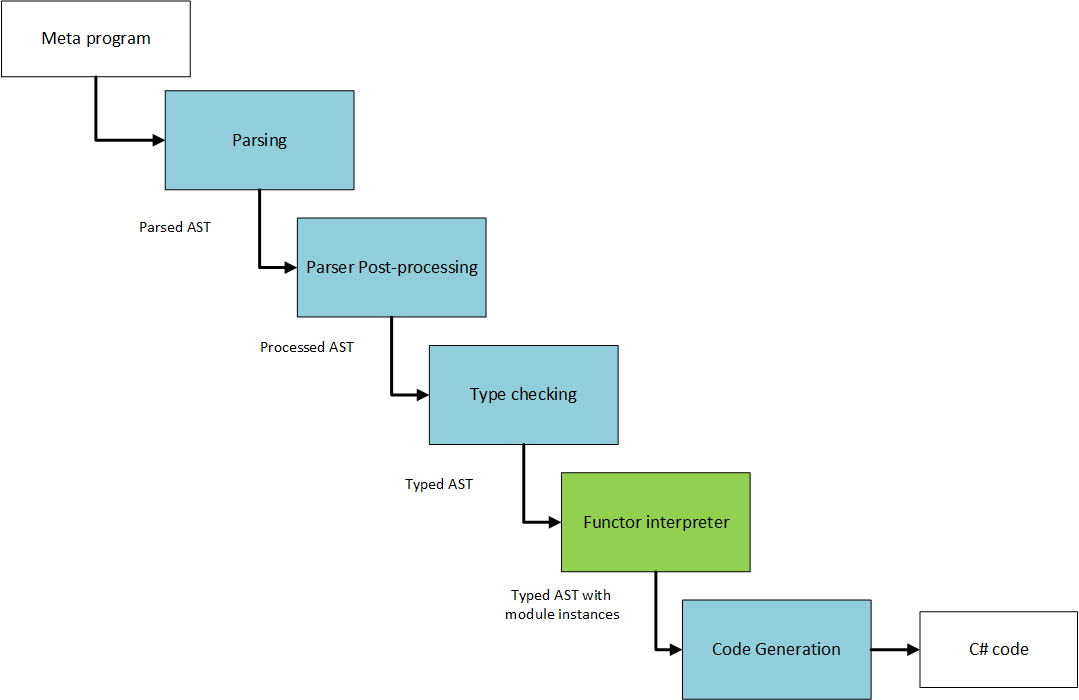
\includegraphics[width=\textwidth]{Figures/chapter_functors/compiler_architecture_functors}
	\caption{Compiler architecture with functor interpreter}
	\label{fig:ch_functors_compiler_architecture}
\end{figure}

\begin{figure}
	\centering
	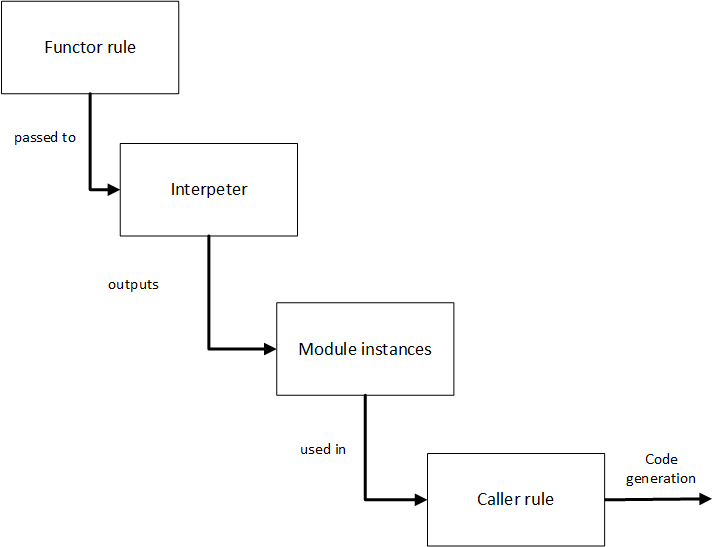
\includegraphics[width=\textwidth]{Figures/chapter_functors/functor_rule_processing}
	\caption{Functor processing}
	\label{fig:ch_functors_functor_processing}
\end{figure}

\section{Record implementation with modules}
\label{sec:ch_functors_record_implementation}
In Section \ref{subsec:ch_functors_inlining} we showed how Casanova entities can be expressed, at meta-language level, as a tuple of field names and values. We also showed that getters and setters always perform the same steps when looking up for the same field because the entity structure does not change at runtime. In this section we proceed to give an implementation based on functors to implement a Casanova entity. We refer to this implementation as ``Record'', since a Casanova entity is simply a record from the point of view of the data representation and since this solution works in general for any data structure that is isomorphic to a record. From now on we also use, as example, the physical body entity described in Section \ref{subsec:ch_functors_casanova_example}.

A module for records simply contains a functor that returns the type of the record. This functor, in general, can return any type since the type of the record can be ``customized'' and depends on the specific definition given by the programmer (thus it cannot be known beforehand). For this reason we use \textit{kind} as return type for this functor. The functor itself is parameterless since nothing is required to generate the type of a record.

\begin{lstlisting}
Module "Record" : Record {
  Functor "RecordType" : * }
\end{lstlisting}

The data representation of the record will be a tuple as shown in Section \ref{subsec:ch_functors_inlining}. For this purpose, we need two functors that are able to represent the type of a record in a recursive way with one being the type of an empty record (a record with no fields) and another a record field followed by the rest of the record representation. The functor for the empty record simply returns the type of the record module, while the functor to represent a record field takes as input a \texttt{string}, representing the name of the field, \textit{kind} because a record field can have any type, and a \texttt{Record} which represents all the other fields coming after the current one. 

\begin{lstlisting}
Functor "EmptyRecord" : Record
Functor "RecordField" => string => * => Record : Record
\end{lstlisting}

After declaring the functors necessary to build a record, we proceed to define their implementation in the form of rules. The functor for an empty record simply generates a module containing a function \texttt{cons}, that is the constructor for the record, that simply returns unit (because an empty record does not contain any field). Consistently, the functor \texttt{RecordType} implemented by the module will simply return \texttt{unit} as type. Note that a module instantiation must implement \textbf{at least} all the declarations of the module (like for an interface), but can add other declarations and implementations that are not shared by all the module instantiations. For example \texttt{cons} for an empty record is different than the one for a non-empty one.

\begin{lstlisting}
-------------------
EmptyRecord => Record {

  Func "cons" : unit
  
  ------------------
  RecordType => unit
  
  ------------------
  cons -> ()

}
\end{lstlisting}

A record field must be constructed through a functor that takes the field name, the type of the field, and the type of the rest of the record. This functor will construct the type of a record as a \texttt{Tuple}, where the first element is the type of the current field and the second the type of the rest of the record. The constructor of the record field will be a function that takes as input an argument of the type of the current field, a tuple representing the remaining part of the record and returns a tuple combining the current field and the rest of the record.

\begin{lstlisting}
------------------
RecordField name type r = Record {
  Func "cons" -> type -> r.RecordType : RecordType

  ---------------------------------------
  RecordType => Tuple[type,r.RecordType]

  -------------------
  cons x xs -> (x,xs)}
\end{lstlisting}

Consider now the physical body representation given above. We show how to use the functors we have just defined to build an instance of a physical body. First of all we defined a functor \texttt{PhysicalBodyType} that returns a \texttt{Record}.

\begin{lstlisting}
Functor "PhysicalBodyType" : Record
\end{lstlisting}

The final representation of the type that should be returned by\\ \texttt{PhysicalBodyType} is \texttt{Tuple[Vector2,Tuple[Vector2,unit]]} because the field \texttt{Position} and \texttt{Velocity} have type \texttt{Vector2}. Note that \texttt{Vector2} can be trivially implemented in Metacasanova as a tuple containing two floating point values. Here we use this type assuming that has already been defined above. The same appiles to \texttt{unit}, which can be defined as a meta-data with no arguments.

The rule to evaluate \texttt{PhysicalBodyType} will call in its premises \texttt{EmptyRecord} and \texttt{RecordField} to generate the type of the tuple appropriately:

\begin{lstlisting}
EmptyRecord => empty
RecordField "Velocity" Vector2 empty => velocity
RecordField "Position" Vector2 velocity => body
----------------------------
PhysicalBodyType => body
\end{lstlisting}

Let us now analyse in detail what the premises generate: the first premise will generate an instance of \texttt{EmptyRecord} and bind it to the variable \texttt{empty}. The instance of this module is parameterless and thus will always be the same every time the functor is invoked. The second premise will instantiate \texttt{RecordField} by using the string \texttt{"Velocity"} as field name, \texttt{Vector2} as field type, and \texttt{empty} as argument for the remaining part of the record (there is no other field after \texttt{Velocity} in the physical body). The instantiation of \texttt{RecordField} produces a rule for the functor \texttt{RecordType}. According to the definition above this functor generates \texttt{Tuple[type,r.RecordType]}. By replacing the argument values provided in the premise, we have 

\begin{lstlisting}
type := Vector2
r := empty := EmptyRecord
\end{lstlisting}

\noindent
Thus \texttt{r.RecordType} uses the functor \texttt{RecordType} in the instance of \texttt{EmptyRecord} which returns the type \texttt{unit} (the call can be seen as \texttt{empty.RecordType}). Thus \texttt{r.RecordType} can be replaced with \texttt{unit}, thus leading to \texttt{Tuple[Vector2, unit]}. Thus the rule for the functor \texttt{RecordType} generated in the module returned by the second premise will be.

\begin{lstlisting}
-----------------------
RecordType => Tuple[Vector2,unit]
\end{lstlisting}

By replacing the argument variables with the values provided in the second premises we can also get the declaration and rule for \texttt{cons}. By replacing again \texttt{type} and \texttt{r.RecordType} as done before, we have that the declaration for \texttt{cons} in the current instance of the module becomes:

\begin{lstlisting}
Func "cons" -> Vector2 -> unit: Tuple[Vector2,unit]
\end{lstlisting}

\noindent
while the corresponding rule will be generated as

\begin{lstlisting}
--------------------
cons x xs -> (x,xs)
\end{lstlisting}

\noindent
The complete module instance will then look like:

\begin{lstlisting}
velocity := Record {
  Func "cons" -> Vector2 -> unit: Tuple[Vector2,unit]
  
  -----------------------
  RecordType => Tuple[Vector2,unit]
  
  --------------------
  cons x xs -> (x,xs)
}
\end{lstlisting}

The third premise calls \texttt{RecordField} with 

\begin{lstlisting}
name := "Position"
type := Vector2
r := velocity
\end{lstlisting}

\noindent
Now in the definition of the \texttt{RecordField} module again the functor \texttt{RecordType} returns \texttt{Tuple[type,r.RecordType]}. Now \texttt{r.RecordType} can be rewritten as \texttt{velocity.RecordType} that returns (see the instantiation of \texttt{velocity} above) \texttt{Tuple[Vector2,unit]}. Thus\\ \texttt{RecordType} for the field \texttt{Position} will be instantiated as

\begin{lstlisting}
-----------------------
RecordType => Tuple[Vector2,Tuple[Vector2,unit]]
\end{lstlisting}

\noindent
Analogously the declaration of \texttt{cons} will be instantiated as

\begin{lstlisting}
Func "cons" -> Vector2 -> Tuple[Vector2,unit]: Tuple[Vector2,Tuple[Vector2,unit]]
\end{lstlisting}

\noindent
while its rule is the same. The full module instance will then be

\begin{lstlisting}
body := Record {
  Func "cons" -> Vector2 -> Tuple[Vector2,unit]: Tuple[Vector2,Tuple[Vector2,unit]]
  
  -----------------------
  RecordType => Tuple[Vector2,Tuple[Vector2,unit]
  
  --------------------
  cons x xs -> (x,xs)
}
\end{lstlisting}

\noindent
which is returned by the functor \texttt{PhysicalBodyType}. In order to build an instance of the physical body, we define a function that returns a value of type \texttt{PhysicalBodyType} (which in turn is simply\\ \texttt{Tuple[Vector2,Tuple[Vector2,unit]}):

\begin{lstlisting}
Func "PhysicalBody" : PhysicalBodyType.RecordType

-----------------------
PhysicalBody -> PhysicalBodyType.cons((10.0,10.0),((10.0,0.0),()))
\end{lstlisting}

\noindent
The rule creates a physical body in position $(10,10)$ moving at velocity $(10,0)$.\\

One of the main arguments in favour of using functors was that they should allow to embed the type system of the embedded language in the meta-type system of Metacasanova. This means that, at compile time, the meta-compiler should be able to detect a physical body that is constructed in the wrong way. Let us then assume that we define another function to build a physical body where the programmer uses a scalar for the velocity instead of a vector:

\begin{lstlisting}
Func "WrongPhysicalBody" : PhysicalBodyType.RecordType

-------------------------------------
WrongPhysicalBody ->  PhysicalBodyType.cons((10.0,10.0),(10.0,()))
\end{lstlisting}

\noindent
What happens is that \texttt{PhysicalBodyType.RecordType} is equal to\\ \texttt{Tuple[Vector2,Tuple[Vector2,unit]]}. At this point the type checker of Metacasanova will successfully match the first element of the tuple returned by the rule, which is correctly provided as a value of type \texttt{Vector2}, but will fail to check the second, which is \texttt{double} where it expects a \texttt{Vector2}. With the implementation based on dictionaries given in Section \ref{subsec:ch_mcnv_languages_casanova_semantics} this check happens dynamically at runtime by means of type rules defined in the meta-program, rather than statically like in this case.

\section{Getting Values from Record Fields}
\label{sec:ch_functors_record_getter}
Getting a value from a record field requires to define a module \texttt{Getter} containing a functor \texttt{GetField} that returns the type of the field that we need to get. This type will be used as the return type of the function\texttt{get} that is able to get that specific field. This function is also contained in this module and takes as argument the record from which we are getting the value and returns, as said above, the value of the field. The module \texttt{Getter} is built using the name of the field that is able to read and the record to read from.

\begin{lstlisting}
Module "Getter" => (name : string) => (r : Record) : Getter { ... }
\end{lstlisting}

The functor \texttt{GetType} returns kind because in general the type of the field of a record is arbitrary. The function \texttt{get} uses in its declaration the functor \texttt{RecordType} to determine the type of the record to use and \texttt{GetType} to determine the type of the field to read. The complete module will look like

\begin{lstlisting}
Module "Getter" => (name : string) => (r : Record) : Getter {
  Functor "GetType" : *
  Func "get" -> (r.RecordType) : GetType
}
\end{lstlisting}

\noindent
The getter has two implementations of the rule that instantiates the \texttt{Getter} module: one is used when the current field in the module tuple is the one we are trying to read, and the other that is able to build the correct getter if the field is in the remaining part of the record. The first happens when the name of the current field is the same as the field name provided as argument of the functor \texttt{GetField}. In this case we have the following rule for the functor:

\begin{lstlisting}
Functor "SetField" => string => Record : Getter
\end{lstlisting}

\begin{lstlisting}[caption = Getting a field (case 1),label = lst:ch_functors_getter1]
name = fieldName
thisRecord := RecordField name type r
--------------------------------------
GetField fieldName (RecordField name type r) => Getter fieldName thisRecord {
  
  ---------------
  GetType => type
  
  ---------------
  get (x,xs) -> x
}
\end{lstlisting}

\noindent
The functor \texttt{GetType} simply returns the type of the current record field, because it is the correct field to read, and \texttt{get} returns the first element of the record tuple, which represents the value stored in the field itself.

When the field we are trying to read is not the one we are currently examining in the record tuple, we must build a getter functor that is able to recursively get the field from the remaining part of the record. At this purpose, we have to extend the \texttt{Getter} with an additional functor \texttt{GetAnotherField} that returns a module instance capable of reading the value from the correct field in the remaining part of the record and its type. The implementation of the rule for this case is the following:

\begin{lstlisting}[caption = Getting a field (case 2),label = lst:ch_functors_getter2]
name <> fieldName
thisRecord := RecordField name type r
-------------------------------------
GetField fieldName (RecordField name type r) => Getter fieldName type thisRecord {
		Functor "GetAnotherField" : Getter
		
		GetField fieldName r => otherGetter
		------------------------------
		GetAnotherField => otherGetter
		
		GetAnotherField => g
		---------------------
		GetType => g.GetType
		
		GetAnotherField => getter
		getter.get xs -> v
		------------------
		get (x,xs) -> v
  }
}
\end{lstlisting}

\noindent
The rule for the functor \texttt{GetAnotherField} simply calls recursively the rule for \texttt{GetField} with the remaining part of the record. If the next field is the correct one then this time we will use the rule in Listing \ref{lst:ch_functors_getter1}, otherwise the rule in Listing \ref{lst:ch_functors_getter2} will be re-applied until the correct field is reached. The functor \texttt{GetType} simply calls \texttt{GetAnotherField} to obtain the module instance necessary to get the field from the rest of the record, and then calls the functor \texttt{GetType} from that instance. Finally, the function \texttt{get} will again use \texttt{GetAnotherField} and then call the \texttt{get} function from the getter returned by \texttt{GetAnotherField} with the remaining part of the record tuple. This function call will return the desired value that will be used also as result of the current \texttt{get}.

Let us now consider again the physical body implemented with functors in Section \ref{sec:ch_functors_record_implementation} and let us assume that we want to get the value of the field \texttt{Position}. We define a function \texttt{getPos} that takes as input a physical body and returns \texttt{Vector2}. This function will use \texttt{GetField} in its premises to generate the getter for \texttt{Position} and will then call the \texttt{get} function from the generated module instance.

\begin{lstlisting}[caption = Getter for the Position field, label = lst:ch_functors_position_getter]
Func "getPos" : Vector2

GetField "Position" PhysicalBodyType => getter
PhysicalBody -> body
getter.get body -> p
-----------------
getPos -> p
\end{lstlisting}

\noindent
Note that in the code above we are using the functor \texttt{PhysicalBodyType} and the function \texttt{PhysicalBody} defined in Section \ref{sec:ch_functors_record_implementation}. Now let us analyse step-by-step what happens when we call \texttt{getPos}. The first premise will call the functor \texttt{GetField} with 

\begin{lstlisting}
fieldName := "Position"
r := PhysicalBodyType := RecordField "Position" Vector2 (RecordField "Velocity" Vector2 EmptyRecord)
\end{lstlisting}

\noindent
At this point the rule for \texttt{GetField} will deconstruct \texttt{RecordField} in its conclusion by means of pattern matching and set 

\begin{lstlisting}
name := "Position"
type := Vector2
r := RecordField "Velocity" Vector2 EmptyRecord
\end{lstlisting}
 
\noindent
Since \texttt{name} = \texttt{fieldName} we fall in the case in Listing \ref{lst:ch_functors_getter1}. Thus we instantiate the module \texttt{Getter} by setting the construction arguments to 

\begin{lstlisting}
name := "Position"
r := RecordField "Position" Vector2 (RecordField "Velocity" Vector2 EmptyRecord)
\end{lstlisting}

\noindent
In this module instance the functor \texttt{GetType} returns \texttt{type :=  Vector2} and \texttt{get} returns the first element of the record tuple. At this point, the third premise will call \texttt{get} from this module instance by passing the record tuple \texttt{((10.0,10.0),((10.0,0.0),()))}, which in turn returns correctly\\ \texttt{(10.0,10.0)}.

Now let us assume that we want to retrieve the value of "Velocity" instead. We define an analogous function \texttt{getVel} as follows

\begin{lstlisting}
Func "getVel" : Vector2

GetField "Velocity" PhysicalBodyType => getter
PhysicalBody -> body
getter.get body -> v
-----------------
getVel -> v
\end{lstlisting}

\noindent
This time the functor \texttt{GetField} is called with

\begin{lstlisting}
fieldName := "Velocity"
r := PhysicalBodyType := RecordField "Position" Vector2 (RecordField "Velocity" Vector2 EmptyRecord)
\end{lstlisting}

\noindent
thus the rule in case 2 is triggered. This rule will generate an instance of \texttt{Getter}

\begin{lstlisting}
fieldName := "Velocity"
type := Vector2
r := RecordField "Velocity" Vector2 EmptyRecord
\end{lstlisting}

\noindent
This rule will generate a module containing the auxiliary functor\\ \texttt{GetAnotherField} that is capable to retrieve the correct field in the remaining part of the record. The rule that processes \texttt{GetAnotherField} will call, in its premise, \texttt{GetField} with

\begin{lstlisting}
fieldName := "Velocity"
r := RecordField "Velocity" Vector2 EmptyRecord
\end{lstlisting}

Since now the name of the field of the getter coincides with the name of the field in \texttt{RecordField}, this premise will now trigger the rule in Listing \ref{lst:ch_functors_getter2} that in turn generates an instance of \texttt{GetField} containing the following:

\begin{lstlisting}[caption = Getter for Velocity generated by \texttt{GetAnotherField}, label = lst:ch_functors_velocity_getter2]
Func "get" -> Tuple[Vector2,unit] : Vector2

-------------------
GetType => Vector2


----------------
get (x,xs) -> x
\end{lstlisting}

\noindent
This module instance will be the one returned by the rule of \texttt{GetAnotherField}. The rule of the functor \texttt{GetType} for \texttt{Velocity} will use \texttt{GetAnotherField} to retrieve the correct field type using the module instance generated in Listing \ref{lst:ch_functors_velocity_getter2} and return it (which is \texttt{Vector2}). The rule for the function \texttt{get} will use \texttt{GetAnotherField} to call the the \texttt{get} function from Listing \ref{lst:ch_functors_velocity_getter2} passing the second element of the record tuple as argument and returns the result of this function call.

Note that the module instantiation will be again performed at compile time, thus the only operations performed at runtime are the calls to the \texttt{get} functions contained in the module instantiations.

\section{Setting Values of Record Fields}
\label{sec:ch_functors_record_setter}
The setter module is analogous to the getter, except that this time the module must generate a function that, in addition to the record, takes as input the value to write in the field. This function returns a modified copy of the record tuple where the value associated to the field has been changed. For this purpose we need a module containing a functor \texttt{SetType} that returns the type of the field to set. This functor will be used to build the declaration of a function \texttt{set} that is able to set the specified field.

\begin{lstlisting}
Module "Setter" => (name : string) => (r : Record) : Setter {
	Functor "SetType" : *
	Func "set" -> r.RecordType -> SetType : r.RecordType
}
\end{lstlisting}

\noindent
The declaration of the function \texttt{set} uses \texttt{r.RecordType} to define the type of the record argument, \texttt{SetType} to define the type of the field to set, necessary for the argument containing the value to set, and returns \texttt{r.RecordType}, which is the modified version of the record.

Analogously to the getter, we need a functor that instantiates \texttt{Setter} and has two different implementations of the instantiation rule: one where the field of the current element of the record tuple coincides with the one we want to set, and the other where the field is different and that is able to build a setter for the remaining part of the record tuple.

\begin{lstlisting}
Functor "SetField" => string => Record : Setter
\end{lstlisting}

The first case is implemented as follows:

\begin{lstlisting}[caption = Setting a field (case 1), label = lst:ch_functors_setter1]
name = fieldName
thisRecord := RecordField name type r
------------------------------
SetField fieldName (RecordField name type r) => Setter fieldName thisRecord {

  ----------------
  SetType => type
  
  ----------------------
  set (x,xs) v -> (v,xs)
}
\end{lstlisting}

\noindent
The function \texttt{SetType} simply returns the type of the field in the current \texttt{RecordField}, while the rule for \texttt{set} replaces the first value in the record tuple with the new value. The second rule is implemented as follows

\begin{lstlisting}[caption = Setting a field (case 2), label = lst:ch_functors_setter2]
name <> fieldName
thisRecord := RecordField name type r
-------------------------------------
SetField fieldName (RecordField name type r) => Setter fieldName thisRecord {
  Functor "SetAnotherField" : Setter
  
  SetField fieldName r => setter
  -------------------------------
  SetAnotherField => setter
  
  SetAnotherField => s
  -------------------------
  SetType => s.SetType
  
  SetAnotherField => setter
  setter.set xs v -> xs'
  --------------------
  set (x,xs) v -> xs'
}
\end{lstlisting}

\noindent
The functor \texttt{SetAnotherField} is an auxiliary functor that recursively calls \texttt{SetField} with the remaining part of the record. Eventually \texttt{SetField} will trigger the rule in Listing \ref{lst:ch_functors_setter1} when the correct field is encountered. This auxiliary functor is then used in \texttt{SetType} to retrieve the correct type of the record field and in the function \texttt{set} to call the correct \texttt{set} function for the field. The \texttt{set} function in the setter generated by \texttt{SetAnotherField} returns a modified version of the record that is replaced in the tuple.

Let us now consider again the physical body and assume that we want to define a setter for \texttt{Position}. Again we define a function \texttt{setPos} for the field:

\begin{lstlisting}
Func "setPos" -> Vector2 : PhysicalBodyType

SetField "Position" PhysicalBodyType => setter
PhysicalBody -> body
setter.set body -> body'
-----------------------
setPos v -> body'
\end{lstlisting}

\noindent
Again we are using the functor \texttt{PhysicalBodyType} and the function\\ \texttt{PhysicalBody} defined in Section \ref{sec:ch_functors_record_implementation}. The first premise of this rule will call \texttt{SetField} with

\begin{lstlisting}
fieldName := "Position"
name := "Position"
type := Vector2
r := RecordField "Velocity" Vector2 EmptyRecord
\end{lstlisting}

\noindent
which, in turn, instantiates \texttt{Setter} with 

\begin{lstlisting}
name := "Position"
r := RecordField "Position" Vector2 (RecordField "Velocity" Vector2 EmptyRecord)
\end{lstlisting}

\noindent
In this module instance \texttt{r.RecordType} will be\\ \texttt{Tuple[Vector2,Tuple[Vector2,unit]]} and \texttt{SetType} returns \texttt{Vector2}. The whole instance will look like

\begin{lstlisting}
Func "set" -> Tuple[Vector2,Tuple[Vector2,unit]] -> Vector2 : Tuple[Vector2,Tupe[Vector2,unit]]

------------------
SetType => Vector2


----------------------
set (x,xs) v -> (v,xs)
\end{lstlisting}

\noindent
Now let us assume that we want to build a setter for \texttt{Velocity}. We have to define a function \texttt{setVel} as follows

\begin{lstlisting}
Func "setVel" -> Vector2 : PhysicalBodyType

SetField "Velocity" PhysicalBodyType => setter
PhysicalBody -> body
setter.set v -> body'
-------------------------
setVel v -> body'
\end{lstlisting}

\noindent
The first premise of this rule will now invoke \texttt{SetField} with

\begin{lstlisting}
fieldName := "Velocity"
name := "Position"
type := Vector2
r := RecordField "Velocity" Vector2 EmptyRecord
\end{lstlisting}

\noindent
which will trigger the rule in Listing \ref{lst:ch_functors_setter2} instead. This will create an instance of \texttt{Setter} containing  the auxiliary functor \texttt{SetAnotherField}. The rule for this functor will call in turn \texttt{SetField} with

\begin{lstlisting}
fieldName := "Velocity"
name := "Velocity"
type := Vector2
r := EmptyRecord
\end{lstlisting}

\noindent
that will generate a different instance of \texttt{Setter}, this time using the rule in Listing \ref{lst:ch_functors_setter1}. The auxiliary setter will contain a functor \texttt{SetType} returning \texttt{Vector2} and a function \texttt{set} that inserts the value for \texttt{Velocity} in the record tuple. The \texttt{set} in the auxiliary setter will be used in the setter of \texttt{Velocity} to obtain the modified copy of the record containing the new value. Again all the modules are generated at compile time, thus the only operations performed at runtime are the calls to the \texttt{set} functions of the field setter and eventual auxiliary modules.

\section{Handling errors in getters and setters}
\label{sec:ch_functors_error_handling}
In Section \ref{sec:ch_functors_record_getter} and \ref{sec:ch_functors_record_setter} we explained how to use functors to implement getters and setters for the fields of a record. The explanation however did not take into account possible mistakes that could be committed during the definition of setters and getters for a specific record.

A possible mistake that could arise in the process of defining getters and setters would be to provide an incompatible type for the \texttt{get} function of a field. For instance, let us assume that we define \texttt{getPos} as

\begin{lstlisting}
Func "wrongGetPos" : double

GetField "Position" PhysicalBodyType => getter
PhysicalBody -> body
getter.get body -> v
-----------------
wrongGetPos -> v
\end{lstlisting}

\noindent
As explained above the getter module will contain a function \texttt{get} that returns a \texttt{Vector2}, because that is the type of the field \texttt{Position}. In the process of building the module, this type is automatically retrieved from the definition of \texttt{PhysicalBodyType}. At this point the meta-compiler would report an error message because this wrong definition of \texttt{getPos} returns \texttt{double} but \texttt{get} returns a \texttt{Vector2}. Note that, as previously explained in Section \ref{sec:ch_functors_record_implementation}, this is possible because functors are able to embed the type system of the embedded language into the Metacasanova type system.


Another possible mistake is accessing a field that is not defined for the record. For instance, let us assume that someone tries to build a getter for a field that does not exist in physical body, namely a field \texttt{Acceleration}. As usual we would define a function for the getter such as

\begin{lstlisting}
Func "getAcc" : Vector2

GetField "Acceleration" PhysicalBodyType => getter
PhysicalBody -> body
getter.get body -> v
---------------
getAcc -> v
\end{lstlisting}

\noindent
The first premise of this rule will call the functor \texttt{GetField} with

\begin{lstlisting}
fieldName := "Acceleration"
name := "Position"
type := Vector2
r := RecordField "Velocity" Vector2 EmptyRecord
\end{lstlisting}

\noindent
As seen above, this rule will generate an auxiliary module by recursively call \texttt{GetField} with

\begin{lstlisting}
fieldName := "Acceleration"
name := "Velocity"
type := Vector2
r : = EmptyRecord
\end{lstlisting}

\noindent
but at this point, since again \texttt{fieldName} $\neq$ \texttt{name} we will recursively call \texttt{GetField}. At this point we will fail to run a suitable rule for the functor, since the only two versions we have so far are able to process \texttt{RecordField} and not \texttt{EmptyRecord}, thus the pattern matching in the conclusion would fail. The meta-compiler will in any case fail to generate code, since the functor evaluation will fail and thus the whole code generation, but this approach is not ``clean'', since the meta-compiler will report a generic error regarding the rule execution failure. An alternative to this, is to include a case for the rule that processes \texttt{EmptyRecord}. A getter for an \texttt{EmptyRecord} returns \texttt{()} and \texttt{GetType} returns the type \texttt{unit}. This rule can be implemented as follows:

\begin{lstlisting}

fieldName <> name
thisRecord := RecordField name type EmptyRecord
-------------------------------
GetField fieldName (RecordField name type EmptyRecord) => Getter fieldName thisRecord {
	
  ----------------
  GetType => unit
  
  ----------------
  get (x,xs) -> ()
}
\end{lstlisting}

In this way the first premise of the rule of \texttt{getAcc} would generate a getter that takes a physical body and returns \texttt{unit}. When the rule calls this getter and returns \texttt{unit}, this will be incompatible with the return type of \texttt{getAcc} that should be a \texttt{Vector2}. The same can be done for \texttt{setAcc}, that is we extend the rule for \texttt{SetField} with an additional case:

\begin{lstlisting}
fieldName <> name
thisRecord := RecordField name type EmptyRecord
--------------------------
SetField fieldName (RecordField name type EmptyRecord) => Setter fieldName thisRecord {
	
	----------------
	SetType => unit
	
	----------------------
	set (x,xs) v -> (x,xs)
}
\end{lstlisting}

\noindent
In this way, when invoking \texttt{set} in the premise \texttt{setAcc} the compiler will signal a type error because at some point it will try to use the \texttt{set} for the \texttt{EmptyRecord} with \texttt{Vector2}. Another alternative, which goes beyond the scope of this chapter, would be to allow rules in meta-casanova to output custom compilation errors. In this way we could write the very same rule case done above but this time we would return a compilation error message reporting that the field does not exist.

\section{Evaluation}
\label{sec:ch_functors_evaluation}
In the previous sections we presented an extension to the meta-language of Metacasanova that allows to embed the type system of an embedded language, whose definition is implemented in Metacasanova, in the meta-type system of Metacasanova. We claimed that this would improve the runtime performance of a program written in the embedded language because we could get rid of all the dynamic checks and accesses to meta-data structures used to implement data structures in the embedded language, such as records. In this section we present the experimental evaluation that should produce the evidence to back up this claim. We proceed to describe the experimental set-up and then we comment the results.

\subsection{Experimental Set-up}
In this experiment we use the implementation of records with functors described in this chapter and we compare its runtime performance with its dynamic counter part, i.e. the implementation that uses dictionaries, that was used to implement the Casanova memory model in Section \ref{subsec:ch_mcnv_languages_casanova_semantics}. The sample measures the run-time of both the functor implementation and the implementation with dynamic tables. We run the test by varying both the amount of record instances and the amount of fields per record. The test is run with a sample of 10000, 100000, and 1000000 record instances and with a number of fields from 1 to 10. We neglect to consider different field types, as the performance of look-up operations is not affected by the type of the fields themselves.

\subsection{Results}

In Table \ref{tab:ch_functors_results}, we can see that the optimization using Functors leads to a performance increase on average of about 11 times, with peaks of 30 times. The gain increases with the number of fields, thus the implementation with functors is particularly effective for records with high number of fields. This is due to the fact that the runtime complexity of a dynamic table depends on the number of entries stored in it (which would be the fields in our case) and thus, when the fields are few, this number is very close to the complexity of the functorial implementation, which is constant. When the amount of fields increases, the performance of the functorial implementation remains the same while the dynamic table one worsens visibly. The constant complexity of the functorial implementation is due to the fact that the meta-compiler builds the functions to look up for a specific field at compile time by generating the appropriate module instances with the functors. The \texttt{get} and \texttt{set} functions described above can either immediately get or set the value of the field and return the result of this operation, or call the getter or setter of an auxiliary module instance that is able to read or write the appropriate field. The only overhead is the overhead of chaining calls to Metacasanova functions, thus the overhead of creating and executing the code that implements the rule behaviour described in Section \ref{sec:ch_metacasanova_code_generation}.

Figure \ref{fig:ch_functors_chart} shows a chart of the overall performance of the two techniques (the data points are taken from Table \ref{tab:ch_functors_results}). The horizontal axis contains the amount of fields per record, while the vertical axis contains the number of records that are being updated. We can see that the performance of the dynamic table degrades considerably when increasing the number of fields, and that the higher the amount of records is, the steeper the curve is. On the other hand, the performance of the implementation with Functors is almost constant, regardless of the amount of fields or records that are being updated. Moreover, note that the performance of the dynamic table is improved by the fact that we are using a dictionary implemented in .NET. If the symbol table were represented as a meta-data structure in the language, the performance would be even worse, since it would have to be encoded as a list of pairs with the field name and its value, and its manipulation would be affected by the evaluation rules that should implement this behaviour. Furthermore, the dynamic lookup should be done also to ensure that the types of the record fields are used consistently (which is not accounted for here, for example to prevent that a record is constructed with incompatible values for its fields), while this check is done at compile time with functors, thus drastically improving the performance

\begin{table}	
	\caption{Running time with the functor optimization and the dynamic table with 10000, 100000, and 1000000 records.}
	\begin{tabular}{|c|c|c|c|}
		\hline
		\textbf{FIELDS}& \textbf{Functors (ms)}&\textbf{Dynamic Table (ms)} & \textbf{Gain}\\ \hline
		1&	1.00E-05&	5.00E-06&	0.50\\ \hline
		2&	9.00E-06&	1.30E-05&	1.44\\ \hline
		3&	9.00E-06&	2.70E-05&	3.00\\ \hline
		4&	9.00E-06&	4.50E-05&	5.00\\ \hline
		5&	9.00E-06&	7.00E-05&	7.78\\ \hline
		6&	9.00E-06&	9.90E-05&	11.00\\ \hline
		7&	9.00E-06&	1.33E-04&	14.78\\ \hline
		8&	9.00E-06&	1.75E-04&	19.44\\ \hline
		9&	9.00E-06&	2.20E-04&	24.44\\ \hline
		10&	9.00E-06&	2.70E-04&	30.00\\ \hline
		\multicolumn{2}{c|}{} & \textbf{Average gain} & 11.74\\ \cline{3-4}			
	\end{tabular}
	
	\vspace{0.15cm}
	\begin{tabular}{|c|c|c|c|}
		\hline
		\textbf{FIELDS}& \textbf{Functors (ms)}&\textbf{Dynamic Table (ms)} & \textbf{Gain}\\ \hline
		1&	9.60E-05&	6.30E-05&	0.66\\ \hline
		2&	9.40E-05&	1.59E-04&	1.69\\ \hline
		3&	9.50E-05&	3.04E-04&	3.20\\ \hline
		4&	9.60E-05&	5.03E-04&	5.24\\ \hline
		5&	9.60E-05&	7.52E-04&	7.83\\ \hline
		6&	9.60E-05&	1.05E-03&	10.95\\ \hline
		7&	9.70E-05&	1.41E-03&	14.57\\ \hline
		8&	9.80E-05&	1.82E-03&	18.59\\ \hline
		9&	9.90E-05&	2.29E-03&	23.17\\ \hline
		10&	1.00E-04&	2.81E-03&	28.05\\ \hline
		\multicolumn{2}{c|}{} & \textbf{Average gain} & 11.39\\ \cline{3-4}						
	\end{tabular}
	
	\vspace{0.15cm}
	\begin{tabular}{|c|c|c|c|}
		\hline
		\textbf{FIELDS}& \textbf{Functors (ms)}&\textbf{Dynamic Table (ms)} & \textbf{Gain}\\ \hline
		1&	9.47E-04&	7.29E-04&	0.77\\ \hline
		2&	9.51E-04&	1.78E-03&	1.87\\ \hline
		3&	9.50E-04&	3.33E-03&	3.51\\ \hline
		4&	9.60E-04&	5.43E-03&	5.66\\ \hline
		5&	9.65E-04&	8.03E-03&	8.32\\ \hline
		6&	9.71E-04&	1.11E-02&	11.44\\ \hline
		7&	9.75E-04&	1.47E-02&	15.12\\ \hline
		8&	9.82E-04&	1.89E-02&	19.28\\ \hline
		9&	9.92E-04&	2.37E-02&	23.86\\ \hline
		10&	1.00E-03&	2.87E-02&	28.62\\ \hline
		\multicolumn{2}{c|}{} & \textbf{Average gain} & 11.84\\ \cline{3-4}						
	\end{tabular}
	\label{tab:ch_functors_results}
\end{table}

\begin{figure}
	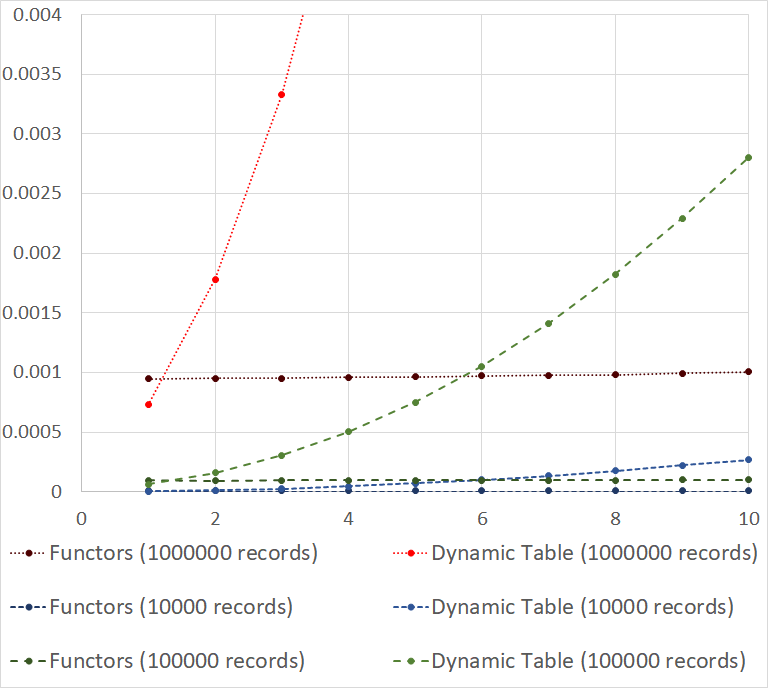
\includegraphics[width = \textwidth]{Figures/chapter_functors/functor_chart}
	\caption{Execution time of the different memory models}
	\label{fig:ch_functors_chart}
\end{figure}

\section{Summary}
In this chapter we addressed the problem arisen in Chapter \ref{ch:mcnv_languages_evaluation} about the performance of the generated code and the forced dynamic behaviour of languages implemented in Metacasanova. We started by informally state that this issue was due to the fact that it was not possible to embed the type system of a language in the meta-type system of Metacasanova, and this caused all the dynamic lookups and accesses at runtime. This could be avoided by using a meta-language abstraction that allows both to define the type system of the embedded language in terms of the meta-type system of Metacasanova and to generate the code for the accesses to the data structures of the embedded language at compile time. At this purpose, we showed a language extension that provides such abstraction in terms of modules and functors. We then proceeded to provide an example of their usage in the context of record getters and setters for their fields. We then measured the performance gain by comparing the implementation with functors with the one using dynamic tables that was employed for the Casanova language implementation shown in Chapter \ref{ch:mcnv_languages_evaluation}. The results show that the performance of operations on records in the case of functors is faster than up to 30 times with respect to the dynamic table implementation. We have also shown that the performance of such operations in the case of functors is constant with respect to the number of fields to update, while the performance of the dynamic table drastically worsens when the number of fields in a record increase. In the next chapter we will show a further example of use of functors to re-implement Casanova semantics and extend the language with abstractions for the networking behaviour of multiplayer games.
